\section{Odd Elastodynamics IV}

We study the overdamped limit:
\begin{equation}
    \Gamma \p_t u_i = F_i = \p_j \sigma_{ij} = \p_j (K_{ijkl}u_{kl}) = K_{ijkl}\p_j\p_l u_k
\end{equation}
In the space of shears:
\begin{equation}
    \Gamma \p_i \m{u_x \\ u_y} = \m{G & -K^0 \\ K^0 & G}\m{\nabla^2 u_x \\ \nabla^2 u_y}
\end{equation}
or in more full generality, after Fourier transforming and looking at the parallel/perpendicular (to the wavevector) components:
\begin{equation}\label{eq:dynamical}
    -i\Gamma \omega\m{u_\parallel \\ u_\perp}  = q^2\m{B + G & K^0 \\ -K^0 - A & G}\m{u_\parallel \\ u_\perp}
\end{equation}
By studying this eigenvalue problem, we get the plot:
\begin{center}
    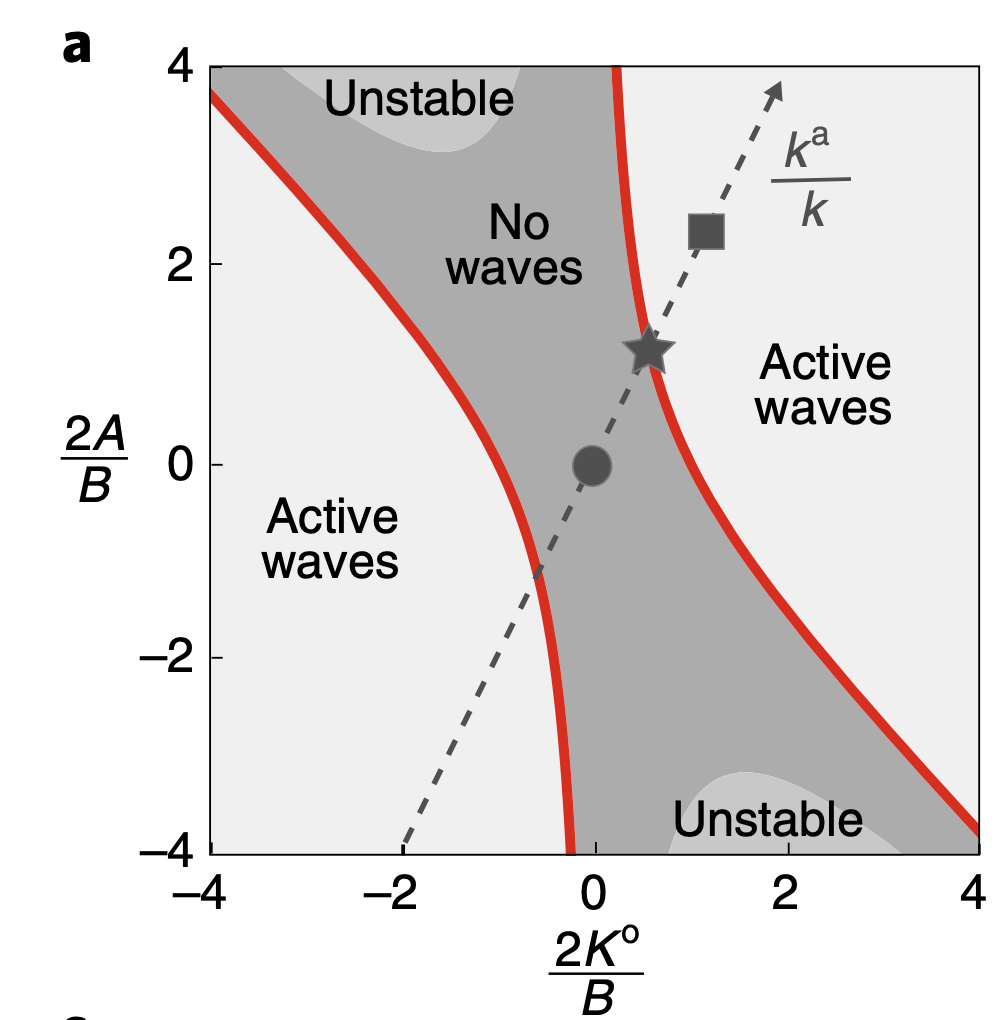
\includegraphics[scale=0.5]{Lectures/Images/lec6-oddelasticphasediagram.png}
\end{center}
We call the propagating waves ``active waves'' as they are propagated by the cycles arising from the odd elastic moduli.

The red lines that separate the regions where the waves do not propagate are called ``exceptional lines'', meaning they consist of exceptional points - the two eigenvalues of the dynamical matrix become degenerate, and the two corresponding eigenvectors become collinear. It is worth noting that the dynamical matrix we have written down in Eq. \eqref{eq:dynamical} is Non-Hermitian (as you may have seen in open quantum systems), and thus the eigenvectors are not orthogonal (and in particular the angle between them goes to zero at the exceptional points).

\subsection{Topological Defects/Dislocations}
We saw some examples last class of auxetic and odd materials. Another system of interest are crystals with topological defects, which exhibit novel behaviour in the presence of stresses. In your homework you do this for the case without odd elastic moduli, but the calculation can also be done in the $K^0 \neq 0$ case, and such behaviour has also been observed by a group at MIT.

In lecture, we watched a video first of rays propagating through a compressed triangular crystal. We then zoomed into it, and saw that it was perfect save for a dislocation where we have made the coordination number 7/5 as opposed to 6. This defect gives rise to an extra row of atoms; for any loop surrounding the defect we are able to detect this extra step. The rays we saw moving through the crystal arose from the ray-like motion of the defects arising from applying a (shear) stress/perturbation to the lattice. 

\begin{center}
    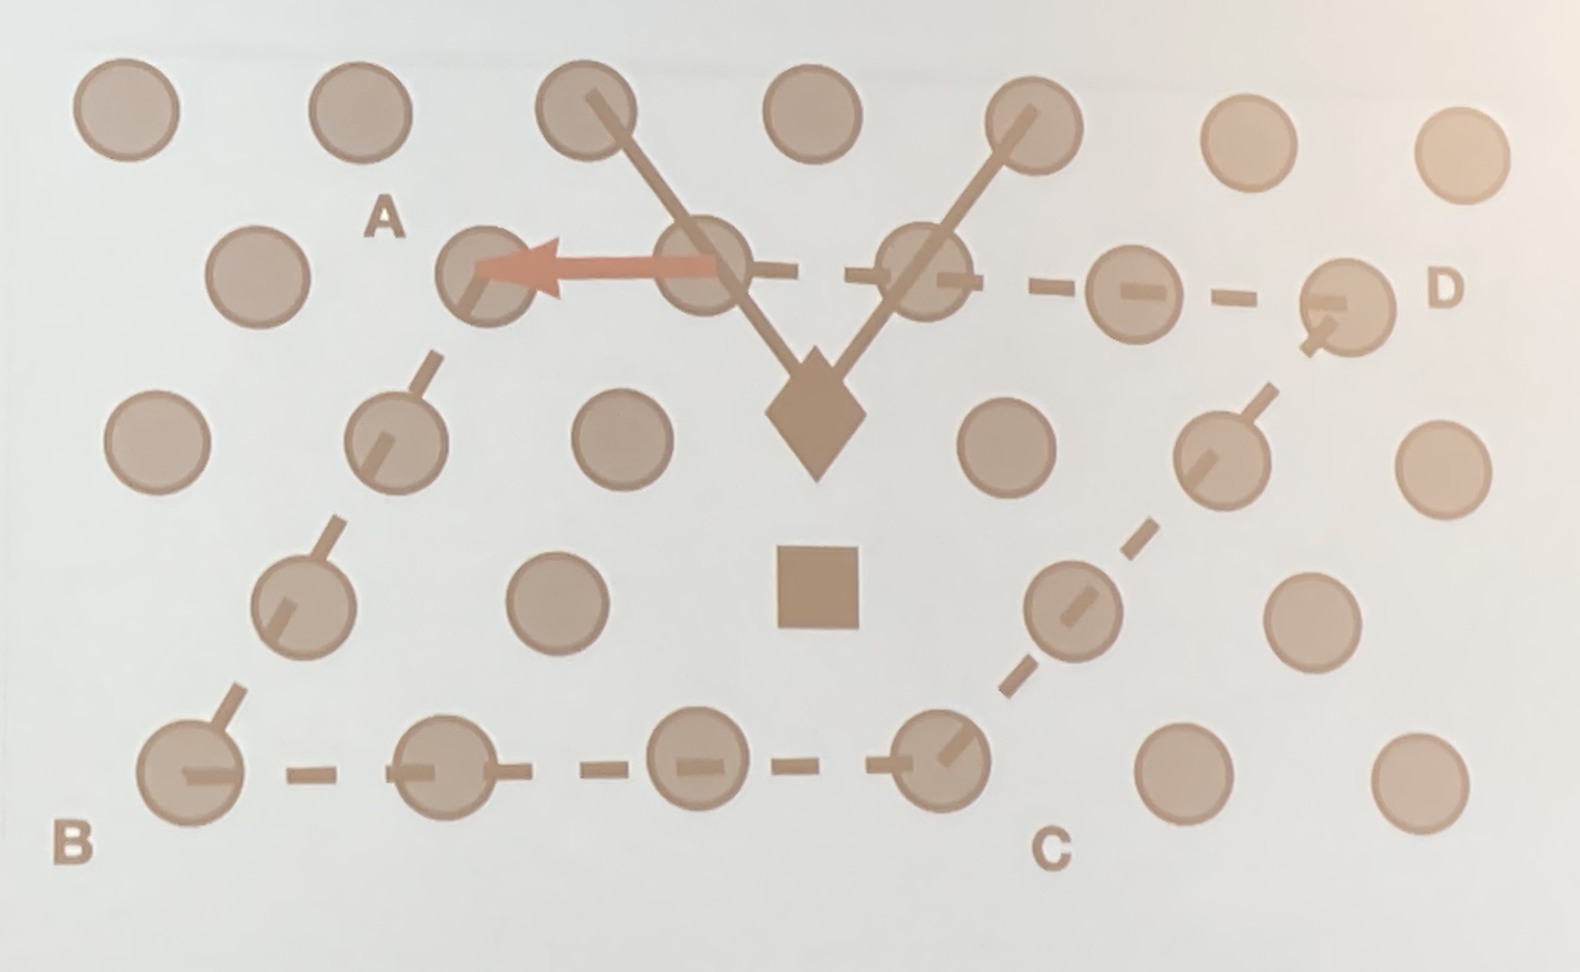
\includegraphics[scale=0.3]{Lectures/Images/lec7-dislocationatoms.png}
\end{center}
Mathematically, the dislocation (which are analogous to magnetic monopoles) is characterized by the Burges vector, where we do a loop integral around the dislocation:
\begin{equation}
    \v{b} = \oint_{\gamma}d\v{r} \cdot \nabla \v{u}
\end{equation}
Then using the force balance condition:
\begin{equation}
    0 = \v{f} = \nabla \cdot \gv{\sigma}
\end{equation}
We have the displacement field:
\begin{equation}
    \v{u}(\v{r}) = \frac{1}{2\pi}\left[\phi \v{b} + \frac{1-\nu}{2}\log(r)\gv{\e} \cdot \v{b} - \frac{1+\nu}{2}\rhat \cdot \v{b}\hat{\gv{\phi}} - \nu^0\left[\log(r)\v{b} + \hat{\gv{\phi}}\cdot \v{b}\hat{\gv{\phi}}\right]\right]
\end{equation}
where the last term is the odd term, with odd ratio:
\begin{equation}
    \nu^0 = \frac{BK^0 - AG}{G(B + G) + K^0(A+K^0)}
\end{equation}
this is zero for a regular crystal (the case you study in your homework), but the odd case was studied theoretically by Lara Braverman and Colin Scheibner, as you can read about in \url{https://journals.aps.org/prl/abstract/10.1103/PhysRevLett.127.268001}. A couple of years later, a team at MIT used the proposal in this Letter to do an experiment with spinning colloids \url{https://www.nature.com/articles/s41586-022-04889-6}, where they tried to extract the odd elastic parameters from the shear angle (though the experimental data is very noisy...).

An equation that we will not derive, but use, is that of the Peach-Koehler (PK) force. It is the analog of the Lorentz force in EM theory:
\begin{equation}
    F_i = q\e_{ijk}v_jB_k
\end{equation}
this is an example of manifest parity violation that you are very familiar with - cyclotron orbits are in a particular direction. There is a mathematically analogous force for dislocations:
\begin{equation}
    F_i^{PK} = -\e_{ij}b_k\sigma_{jk}
\end{equation}
which tells you about the force on the dislocation (characterized by the Burges vector $\v{b}$) as a result of an applied stress. This force is highly orientation dependent.

The crucial feature of the experimental results using spinning colloids is that there are pre-torques/stresses (which violate angular/linear momentum conservation) in $\sigma_{ij}$:
\begin{equation}
    \sigma_{ij} = \underbrace{\tau_0 \e_{ij}}_{\text{pre-torque}} + \underbrace{p\delta_{ij}}_{\text{pre-stress}} + K_{ijkl}\p_k u_l
\end{equation}
If we put the pre-torque into the PK force equation:
\begin{equation}
    F_i^{PK} = -\e_{ij}b_k\tau^0\e_{jk} = \delta_{ik}b_k\tau^0
\end{equation}
where we have used $-\e_{ij}\e_{jk} = \delta_{ik}$. So, we have a force along the direction of the Burges vector, proportional to the pre-torque density $\tau^0$.

One last comment that we won't have time for - in the Braverman/Scheibner PRL, we have formulas are derived from continuum mechanics - but the Burges vector is a dislocation arising from meso/microscopic phenomena. These details can actually lead to the breakdown of the field-theoretic description, and lead to a reversal in the direction of the force as predicted by the field theory formula. Sometimes we can learn as much from the cases where field theory holds, as well as where it breaks down! In particular, here the field theoretic description holds if defects interact at far field, but breaks down if defects become close.

\subsection{Relaxing linear momentum conservation}
All of our discussion thus far has arose because we relaxed the assumption of energy conservation. However, throughout we have been assuming:
\begin{equation}
    F_i = \p_j \sigma_{ij}
\end{equation}
which assumes that the medium conserved linear momentum (the above is the divergence of a flux of linear momentum). This is what gave rise to the force being the second spatial derivative of the displacement/strain.

However, it is possible to write a more general force law, if we relax the conservation law. Let us expand $F_i$ in a general way, expanding in gradients of the deformation:
\begin{equation}
    F_i = \alpha u_i + \beta_{ijk}\p_j u_k + K_{ijkl}\p_j \p_l u_k
\end{equation}
Let's consider a simple solid that violates Newton's third law\footnote{There is a 2025 PNAS paper by Bartolo, Vitelli, Irvine and others that discusses this - and the classification of $\beta_{ijk}$, if you wanted to read more about it.}. We want no adhesion forces, so we drop the first term:
\begin{equation}
    F_i = \beta_{ijk}\p_j u_k + K_{ijkl}\p_j \p_l u_k
\end{equation}
This could be, for example, a fluid that moves through a collection of colloids/droplets. This clearly violates Newton's third law because there is a preferred direction/the colloids feel different forces against/along the fluid flow. A toy model that can describe this would be a chain of 1D masses connected by non-reciprocal (asymmetric) springs:

\begin{center}
    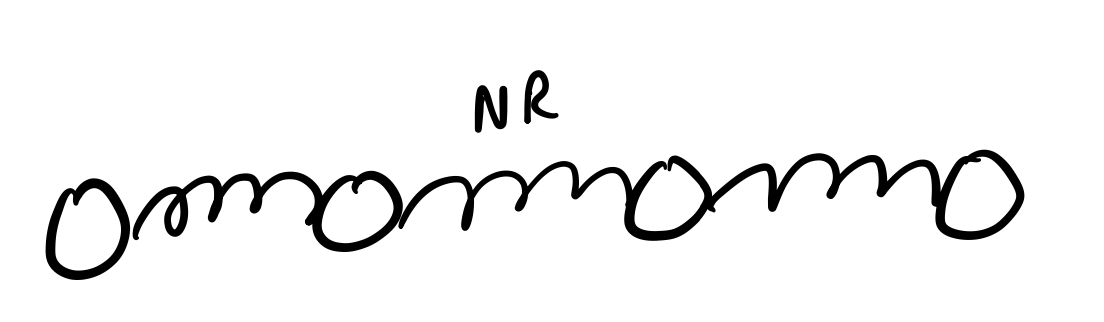
\includegraphics[scale=0.4]{Lectures/Images/lec7-NRspringchain.png}
\end{center}

In this 1-D case, the equation of motion reduces to (still working in the overdamped limit):
\begin{equation}\label{eq:neweom}
    \gamma \p_t u = \beta \p_x u + \kappa \p_x^2 u
\end{equation}
simple as this looks, this is still quite different from the standard wave equation that is studied in the context of solids:
\begin{equation}
    \rho \p_t^2 u = \kappa \p_x^2 u
\end{equation}
wherein the speed of sound is $c = \sqrt{\frac{\kappa}{\rho}}$. The fourier transform of this yields the dispersion relation:
\begin{equation}
    \omega^2 = c^2q^2 = \kappa q^2
\end{equation}
(Where we work in units where $\rho = 1$), or:
\begin{equation}
    \omega(q) = \sqrt{\kappa}\abs{q}
\end{equation}
Note then that:
\begin{equation}
    \omega(q) = \omega(-q)
\end{equation}

Let's also try studying the spectrum for Eq. \eqref{eq:neweom}; fourier transforming (equivalently, using the wave ansatz $u(x, t) = Ae^{i(qx + \omega t)}$). We find:
\begin{equation}
    \gamma i \omega = i q \beta - \kappa q^2
\end{equation}
Or multiplying by $-\frac{i}{\gamma}$:
\begin{equation}
    \omega = \frac{\beta}{\gamma}q + i\frac{\kappa}{\gamma}q^2
\end{equation}

There is a propagating wave term coming from $\frac{\beta}{\gamma}q$, and there is a piece that is attenuating $i\frac{\kappa}{\gamma}q^2$. The part that should draw your attention is that $\omega(q)$ - is \emph{not} invariant under $q \leftrightarrow -q$. Indeed in the $\kappa \to 0$ limit $\omega(q)$ is actually odd under this transformation:
\begin{equation}
    \omega(q) = -\omega(-q)
\end{equation}
The non-reciprocity/breaking of mirror symmetry is what enables this strange feature of the spectrum.